\documentclass[tikz,border=8pt]{standalone}
% Shared look for every TikZ diagram. Load with \input{../../tools/tikz-style.tex}
\usepackage[sfdefault]{roboto}
\usetikzlibrary{arrows.meta, positioning, shapes.geometric, calc, fit, backgrounds}
\definecolor{cblue}{HTML}{4C78A8}
\definecolor{corange}{HTML}{F58518}
\definecolor{cgreen}{HTML}{54A24B}
\definecolor{cred}{HTML}{E45756}
\definecolor{cpurple}{HTML}{B279A2}
\definecolor{cgrey}{HTML}{6B6B6B}
\tikzset{
  every picture/.style={font=\sffamily, line width=1.2pt},
  box/.style={draw=#1, fill=#1!12, rounded corners=4pt, align=center, inner sep=7pt, minimum height=1.1cm},
  box/.default=cgrey,
  arrow/.style={-{Stealth[length=3mm]}, draw=cgrey, line width=1.4pt},
  title/.style={font=\sffamily\bfseries\Large},
  note/.style={font=\sffamily\small, text=cgrey, align=center},
}
\AtBeginDocument{\hyphenpenalty=10000 \exhyphenpenalty=10000}

% The block diagram of the robot's speed loop: reference, summing junction, error, controller, actuator,
% disturbance, plant, output, sensor, sensor noise, measured output. Values from speedkit.py.
\begin{document}
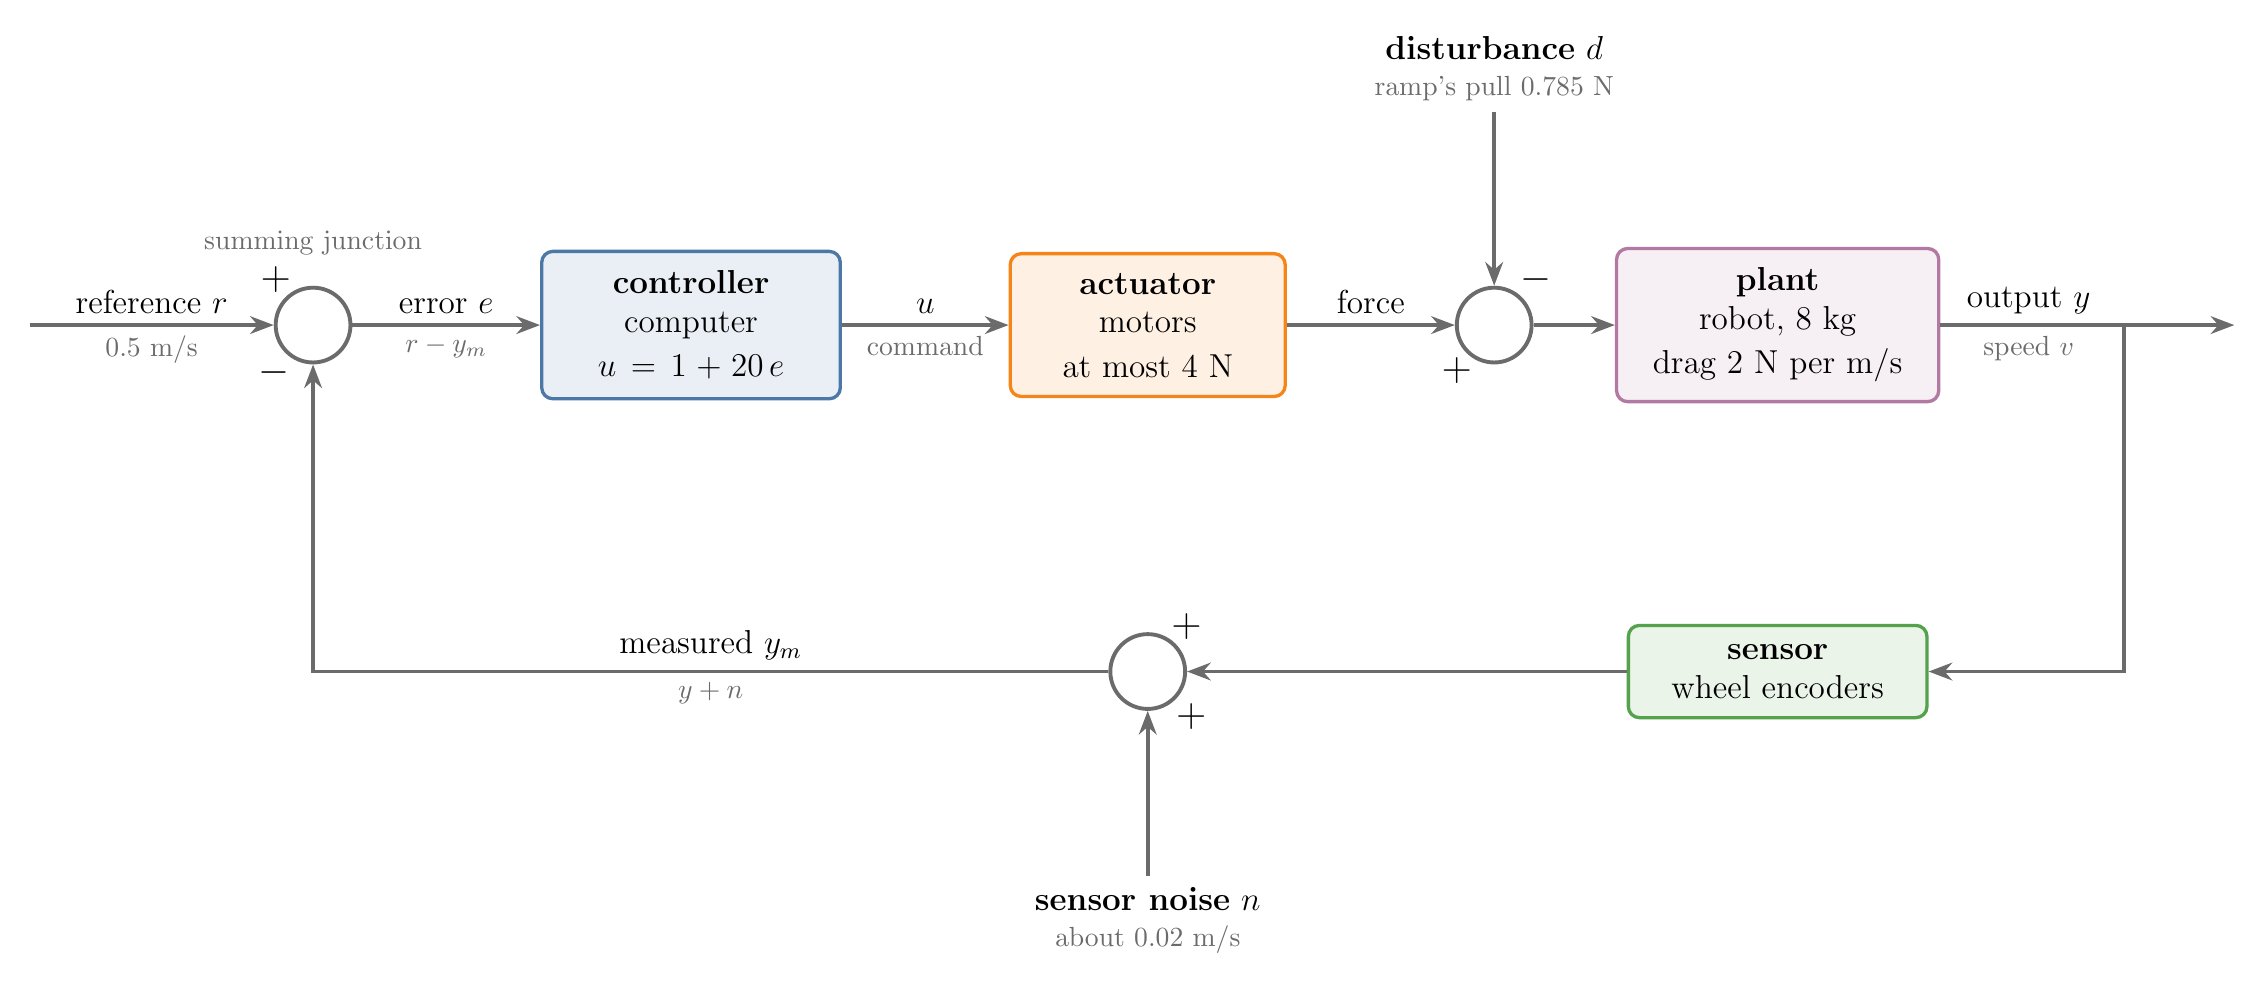
\begin{tikzpicture}[every node/.append style={font=\large},
    sum/.style={circle, draw=cgrey, fill=white, minimum size=0.95cm, inner sep=0pt, line width=1.4pt},
    val/.style={font=\normalsize, text=cgrey, align=center}]
  % top row: forward path
  \node[sum] (s1) at (2.6,0) {};
  \node[box=cblue, text width=3.3cm] (ctrl) at (7.4,0) {\textbf{controller}\\ computer\\[2pt] $u = 1 + 20\,e$};
  \node[box=corange, text width=3.0cm] (act) at (13.2,0) {\textbf{actuator}\\ motors\\[2pt] at most 4 N};
  \node[sum] (s2) at (17.6,0) {};
  \node[box=cpurple, text width=3.6cm] (plant) at (21.2,0) {\textbf{plant}\\ robot, 8 kg\\[2pt] drag 2 N per m/s};
  % bottom row: feedback path
  \node[box=cgreen, text width=3.3cm] (sens) at (21.2,-4.4) {\textbf{sensor}\\ wheel encoders};
  \node[sum] (s3) at (13.2,-4.4) {};
  % reference in
  \draw[arrow] (-1.0,0) -- node[above] {reference $r$} node[below, val] {0.5 m/s} (s1.west);
  \node[font=\Large] at ($(s1.north west)+(-0.12,0.22)$) {$+$};
  \node[font=\Large] at ($(s1.south west)+(-0.14,-0.25)$) {$-$};
  \draw[arrow] (s1.east) -- node[above] {error $e$} node[below, val] {$r - y_m$} (ctrl.west);
  \draw[arrow] (ctrl.east) -- node[above] {$u$} node[below, val] {command} (act.west);
  \draw[arrow] (act.east) -- node[above] {force} (s2.west);
  \node[font=\Large] at ($(s2.south west)+(-0.12,-0.22)$) {$+$};
  \node[font=\Large] at ($(s2.north east)+(0.18,0.22)$) {$-$};
  \draw[arrow] (17.6,2.7) node[above, align=center] {\textbf{disturbance} $d$\\[-1pt] \normalsize\textcolor{cgrey}{ramp's pull 0.785 N}}
     -- (s2.north);
  \draw[arrow] (s2.east) -- (plant.west);
  \draw[arrow] (plant.east) -- node[pos=0.3, above] {output $y$} node[pos=0.3, below, val] {speed $v$} (27.0,0);
  % feedback
  \draw[arrow] (25.6,0) -- (25.6,-4.4) -- (sens.east);
  \draw[arrow] (sens.west) -- (s3.east);
  \node[font=\Large] at ($(s3.north east)+(0.14,0.22)$) {$+$};
  \node[font=\Large] at ($(s3.south east)+(0.2,-0.22)$) {$+$};
  \draw[arrow] (13.2,-7.0) node[below, align=center] {\textbf{sensor noise} $n$\\[-1pt] \normalsize\textcolor{cgrey}{about 0.02 m/s}}
     -- (s3.south);
  \draw[arrow] (s3.west) -- node[above] {measured $y_m$} node[below, val] {$y + n$} (2.6,-4.4) -- (s1.south);
  % the summing junctions named once
  \node[val, anchor=south] at (2.6,0.75) {summing junction};
\end{tikzpicture}
\end{document}
